\chapter{Grundlagen}
\label{chap:basics}
\todo[size=\small, color=yellow!40, inline]{Kapitel: Non-Tim understanding}%
\todo[size=\small, color=yellow!40, inline]{Kapitel: Human proofreading}%
\todo[size=\small, inline]{Evtl. besseren Namen für Kapitel "`Grundlagen"' finden $\rightarrow$ Grundlegende Algorithmen/Techniken?!}%
An dieser Stelle soll zunächst ein Überblick über die in der vorliegenden Arbeit verwendeten Techniken gegeben werden. Diese beinhalten unter anderem Algorithmen der Computergrafik, verwendete Datenstrukturen und die Organisation der Speicherverwaltung.

\section{Datenstrukturen}
\label{sec:basics:datenstrukturen}
3D-Modelle aus Computer Aided Design - Anwendungen (CAD) werden üblicherweise nach ihrer Funktion gruppiert. Das mag beim Entwurf solcher Systeme auch praktisch sein, bei der Visualisierung kann dies jedoch zu Problemen führen. Bei CAD-Modellen in Größenordnung der Boeing 777\footnote{\todo[size=\small, inline]{Boeing Herkunftshinweis verschieben an die erste Stelle wo es erwähnt wird.}%
Das 3D-Modell der Boeing 777 wurde freundlicherweise zur Verfügung gestellt von The Boeing Company, Seattle, WA, USA.} (ca. 350 Millionen Dreiecke) ist es wichtig, dass diese in eine geeignete räumliche Unterteilung überführt werden. Da ein Out-Of-Core-Renderer entwickelt wurde, findet ein ständiges Laden und Verwerfen von Teilmodellen statt. Je länger ein Renderer benötigt, um herauszufinden, welche Teile des Modells er verwerfen kann und welche er als erstes anfordern sollte, desto länger braucht er auch um ein Bild zu erstellen. In dieser Arbeit wurde als hierarchische räumliche Unterteilung ein Randomized Sampletree (\ref{sec:basics:sampletree}) und zum Vergleich ein Loose Octree gewählt.

\subsection{Loose Octree}
\label{sec:basics:octree}
Um einen Octree\footnote{\cite{RTR3}, Seiten 647 ff.} zu erzeugen, wird die gesamte Szene in eine minimale Boundingbox eingeschlossen. Rekursiv wird diese Box entlang der drei räumlichen Achsen in der Mitte geteilt, woraus sich jeweils acht gleich-große Boundingboxen ergeben. Dieser Vorgang wird so lange wiederholt, bis ein Haltekriterium erfüllt ist. Im Falle der Boeing wurde festgelegt, dass höchstens 5.000 Dreiecke in einer Box liegen dürfen und die maximale Tiefe des Baums wurde auf 14 beschränkt. 5.000 Dreiecke stellen im Allgemeinen eine gebräuchliche Geometriegröße für aktuelle Grafikhardware dar. Die maximale Baumtiefe bot sich zu Beginn der Arbeit als ein gutes Maß an, um die häufige Traversion des Baums nicht zu aufwendig werden zu lassen. Dies stellte sich im Nachhinein als Fehler heraus, wurde jedoch aufgrund der Datenmenge dabei belassen (siehe Kapitel \ref{sec:impl:preprocessing}).\\
Erfüllt ein Octree-Knoten eines dieser Kriterien, wird nicht weiter unterteilt. So entstehende, leere Blattknoten, werden entfernt, sodass im fertigen Octree jeder Blattknoten Daten enthält. In Abbildung \ref{fig:basics:octree} ist ein Octree zu sehen. Beim Rendern der Szene wird in jedem Frame der Octree traversiert, um ein Frustum-Culling durchzuführen (siehe auch \ref{sec:basics:algos}). Durch den hierarchischen Aufbau des Baums, ist es möglich die Traversion abzubrechen, fall sich ein Knoten vollständig innerhalb oder außerhalb des Frustums befindet.

\begin{figure}
 \centering
  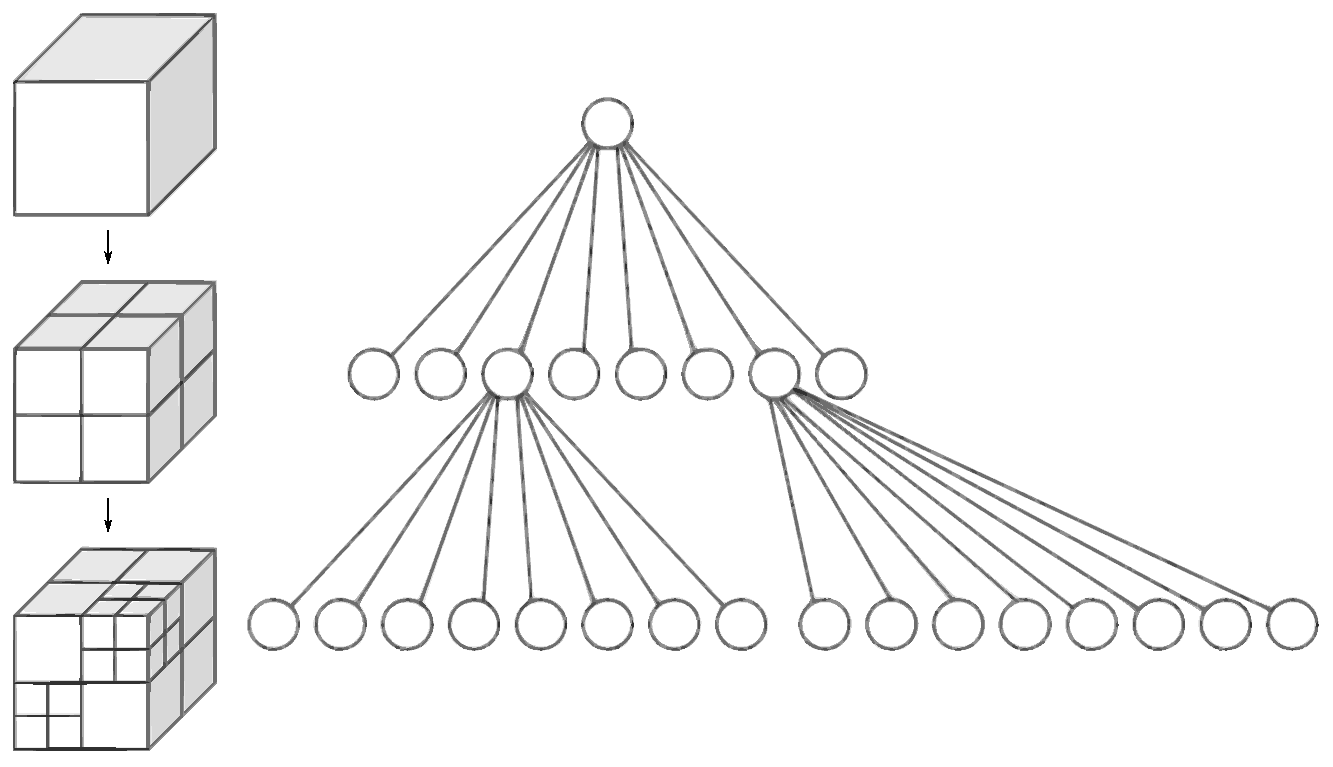
\includegraphics[scale=0.5]{images/octree.pdf}
 % octree.pdf: 640x368 pixel, 72dpi, 22.58x12.98 cm, bb=0 0 640 368
  \caption{Ein Octree der Tiefe 2. \textit{links: die räumliche Darstellung, rechts: die Baumdarstellung. Quelle: \cite{wikioctree}}}
 \label{fig:basics:octree}
\end{figure}
In dieser Arbeit wurde jedoch eine spezielle Form des Octrees verwendet: der Loose Octree. Dieser erweitert den Octree um eine weitere Box pro Knoten: die sogenannte Loosebox. Sie teilt sich ihr Zentrum mit der Octree-Boundingbox, besitzt aber doppelte Kantenlängen. Wird nun festgestellt, dass in einem Knoten mehr als 5.000 Dreiecke liegen, wird die Größe der einzelnen Dreiecke anhand der Looseboxen der Kindknoten geprüft. Liegt ein Dreieck vollständig in der Loosebox mit seinem Zentrum in der eigentlichen Boundingbox des Kindknotens, kann es in den Knoten verschoben werden. Ist dies nicht der Fall, bleibt das Dreieck im aktuellen Knoten (Abbildung \ref{fig:basics:looseoctree}).\\
Dies hat den Vorteil, dass große Dreiecke relativ weit oben im Baum zu liegen kommen und Kleinere entsprechend tief. Es ist anzunehmen, dass größere Dreiecke häufiger sichtbar sind und gezeichnet werden müssen, als kleinere Dreiecke. So lange man sich innerhalb der Szene bewegt, ist der Wurzelknoten beziehungsweise die Szenen-Boundingbox praktisch immer sichtbar, was bedeutet, dass die zur Wurzel gehörige Geometrie gezeichnet werden muss.
\begin{figure}
 \centering
  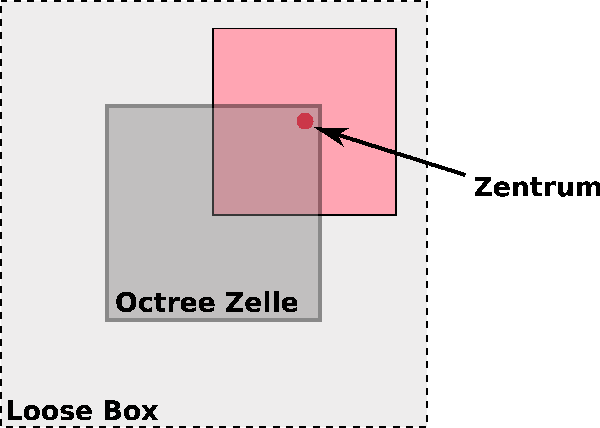
\includegraphics[scale=0.8]{images/looseoctree2.pdf}
  \caption{Ein Loose Octree in einer 2D-Darstellung. \textit{Das Zentrum des Objekts (rosa) befindet sich innerhalb der Octree Zelle, das gesamte Objekt befindet sich innerhalb der Loose Box. Quelle: nach \cite{anteru}}}
 \label{fig:basics:looseoctree}
\end{figure}

\subsection{Randomized Sampletree}
\label{sec:basics:sampletree}
Als spezielle Ausprägung eines Loose Octrees gibt es den Randomized Sampletree \cite{klein}. Dieser unterscheidet sich von einem Octree darin, dass zufällig einzelne Dreiecke aus tieferen Knoten in höhere Knoten verschoben werden. Während des Renderings wird die Baumtraversion abgebrochen, wenn die Entfernung des Knotens zur Kamera einen Schwellwert überschreitet, oder wenn die Größe der im Knoten enthaltenen Dreiecke einen Schwellwert unterschreitet. Dadurch kommt es allerdings zu Darstellungsfehlern, da nicht die gesamte sichtbare Geometrie gerendert wird. Dadurch, dass zufällige kleinere Dreiecke in höher liegenden Knoten gespeichert sind, werden diese auch gerendert. Ist die projizierte Flächensumme alle Dreiecke in einem Knoten des Sampletrees nicht größer als ein Pixel, wird die Traversion abgebrochen. Klein, Krokowski und Fischer \cite{klein} haben gezeigt, dass diese Geometrieapproximation von weit entfernten Objekten durch zufällige Dreiecke eine hinreichend korrekte Darstellung liefert. Dieses Verfahren wurde für komplexe geometrische Umgebungen entwickelt, weshalb es in dieser Arbeit verwendet wurde.
\begin{figure}
 \centering
  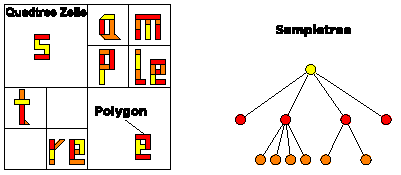
\includegraphics[scale=1.7]{images/sampletree2.pdf}
  \caption{Ein Sampletree in einer 2D-Darstellung. \textit{links: eine Aufteilung von Polygonen in verschiedene Quadtree Zellen. rechts: die Baumdarstellung des Sampletrees. Die farbigen Knoten geben an, welche Polygonteile der linken Seite in welchen Knoten gespeichert wurden. Quelle: nach \cite{klein}}}
 \label{fig:basics:sampletree}
\end{figure}

\section{Computergrafik}
\label{sec:basics:computergrafik}
Da der Speicher einer Grafikkarte in der Regel kleiner als der Arbeitsspeicher ist, werden nicht alle geometrischen Objekte auf der Grafikkarte belassen. Wenn angeforderte Objekte bei einem Renderer eintreffen, werden die zunächst gar nicht an die Grafikkarte geschickt. Erst nach weiteren Überprüfungen, ob das Objekt immer noch sichtbar ist, findet der Transfer zur GPU statt. Dort verbleiben sie dann, bis sie irgendwann aus Platz- oder Sichtbarkeitsgründen verdrängt werden (siehe auch \ref{sec:basics:speicher}). Um dies möglichst effizient umsetzen zu können, werden hier Vertexbuffer Objects (VBOs) genutzt. Die Idee ist dabei, dass Modelldaten, bestehend aus Vertices und Vertex-Normalen, in einem zusammenhängenden Speicherblock abgelegt werden. Ein Vertex besteht aus einer 3D-Koordinate und einer Vertex-Normalen. Der Zugriff auf Dreiecke erfolgt dann mittels einer Indexliste, bei der immer drei Indizes ein Dreieck ergeben. Alle Dreiecke eines Octree-Knotens wurden zu einem Vertexbuffer-Objekt zusammengefasst (siehe \ref{sec:basics:octree}), da Geometrie innerhalb eines Knotens nicht weiter unterteilt wird. In Form von VBOs kann entsprechender Platz im Grafik-RAM reserviert und die Daten in den Speicher geladen werden. Allerdings gibt es gibt keine Garantie dafür, dass der reservierte Speicherbereich tatsächlich im schnellen RAM der Grafikkarte liegt.\\
Im Gegensatz dazu verbleiben bei Vertex-Arrays alle Daten im Arbeitsspeicher des Rechners und werden für jeden Zeichenaufruf zur Grafikkarte übertragen. Vertex-Arrays bieten sich an, wenn Objekte nur einmal gezeichnet und dann verworfen werden. Von daher kommen sie nur auf den Datenknoten (siehe \ref{sec:impl:netzwerkarchitektur}) zum Einsatz, da diese ein getestetes Objekt nur in ihrem Tiefenbuffer rendern und dann wieder verwerfen. Bei VBOs wäre der Overhead der Datenübertragung und der anschließenden Deallokation zu groß für eine einmalige Verwendung.
\begin{figure}
  \centering
  %%%%%%%%%%%%%%%%%%%%%%%%%%%%%%%%%%%%%%%%%%%%%%%%%%%%%%%%%
% 1D-Farbtextur mit Beschreibung und Labels
%%%%%%%%%%%%%%%%%%%%%%%%%%%%%%%%%%%%%%%%%%%%%%%%%%%%%%%%%


\begin{tikzpicture}
  \tikzset{ 
    every pin/.style={fill=yellow!50!white,rectangle,rounded corners=3pt,font=\small}, 
    small dot/.style={fill=black,circle,scale=0.3} } 
  \begin{axis}[
    x=13cm, y=1.0cm, 
    clip=false,
    ytick=\empty,
    xtick={0,0.03125,0.0625,0.09375,0.125,0.15625,0.1875,0.21875,0.25,0.28125,0.3125,
      0.34375,0.375,0.40625,0.4375,0.46875,0.5,0.53125,0.5625,0.59375,0.625,
      0.65625,0.6875,0.71875,0.75,0.78125,0.8125,0.84375,0.875,0.90625,0.9375,
      0.96875,1},
    xticklabels={$0$,$\frac{1}{n}$,$\frac{2}{n}$,$\frac{3}{n}$,$\frac{4}{n}$,$\frac{5}{n}$,$\frac{6}{n}$,$\frac{7}{n}$,$\frac{8}{n}$,$\frac{9}{n}$,$\frac{10}{n}$,
      $\frac{11}{n}$,$\frac{12}{n}$,$\frac{13}{n}$,$\frac{14}{n}$,$\frac{15}{n}$,$\frac{16}{n}$,$\frac{17}{n}$,$\frac{18}{n}$,$\frac{19}{n}$,$\frac{20}{n}$,
      $\frac{21}{n}$,$\frac{22}{n}$,$\frac{23}{n}$,$\frac{24}{n}$,$\frac{25}{n}$,$\frac{26}{n}$,$\frac{27}{n}$,$\frac{28}{n}$,$\frac{29}{n}$,$\frac{30}{n}$,
      $\frac{31}{n}$,$\frac{32}{n}$},
       %tickpos=right,
    major tick length={0.07cm},
    xtick align=outside,
    xtick pos=left,
    tick style={very thin, black},
    tick label style={
    font=\tiny},
    %major x tick num=5,
    %hide y axis,
    enlargelimits=false,
    axis on top] 
    \addplot graphics [xmin=0,xmax=1,ymin=0,ymax=1, 
      % trim=left bottom right top 
      includegraphics={trim=0 9 0 8,clip}
      ] 
      {images/colors.pdf}; 

\node[small dot,pin=-90:{$\frac{1}{2n}$}] at (axis description cs:0.017625,0) {}; 
%\node[small dot,pin=-45:{$\frac{1}{n}$}] at (axis description cs: 0.03325,0) {}; 

  \end{axis} 
\end{tikzpicture}

  \caption{1D-Farbtextur. $n=$Anzahl Farben. Um mittig auf den Texel der Farbe $i$ zuzugreifen, errechnet sich die Texturkoordinate durch $\frac{i}{n}-\frac{1}{2n}$. }
  \label{fig:basics:1dtexture}
\end{figure}

Das Modell der Boeing 777 besitzt auch Farbinformationen. Da bei CAD-Modellen Farben oft einen Hinweis auf den Produktionsort oder auf Komponentengruppen geben, ist die Anzahl der Farben beschränkt. Man könnte jedem Vertex eine Farbe zuordnen. Dies hätte jedoch zur Folge dass bei jedem Vertex die Farbe neu gesetzt werden muss, unabhängig davon, ob diese Farbe bereits gesetzt ist. Dadurch wären die Farben jedoch fest mit dem Modell verbunden. Stattdessen wurde lediglich eine Texturkoordinate als Farbindex genutzt. Die Farbpalette ist somit beliebig austauschbar. Die 32 Farben der Boeing wurden in einer 1D-Textur codiert und die Texturkoordinate wurde als vierte Komponente an den Vertex gehängt. Wird nun ein Vertex gezeichnet, ersetzt der Vertex-Shader die harmonische vierte Komponente eines Vertices wieder durch $1.0$\footnote{Die Beschaffenheit der harmonischen Komponente ist implementierungsabhängig. Bei OpenGL ist diese im Normalfall $1.0$, da in der Modelview-Projection-Matrix Rotation, Translation und Skalierung zusammengefasst sind und andere Werte den Vertex verschieben würden.} und gibt die Textur-Koordinate an den Fragment-Shader weiter. Letzterer muss eine Farbe schreiben, weshalb diese aus der Textur ausgelesen wird. Da die Anzahl der Farben bekannt ist, ergibt sich zur Berechnung der Texturkoordinate der $i$-ten Farbe $\frac{i}{n}-\frac{1}{2n}$ (Abbildung \ref{fig:basics:1dtexture}). Die Subtraktion der Hälfte eines Texels $\frac{1}{2n}$ ist notwendig, da man sonst genau auf die Kante zwischen zwei Farben zugreift, was zu undefiniertem Farbverhalten in der Grafikkarte führt.

\section{Algorithmen}
\label{sec:basics:algos}
In der vorliegenden Arbeit wurden verschiedene Algorithmen benutzt, welche an dieser Stelle näher erklärt werden sollen.

\subsection{Culling}
\label{sec:basics:algos:culling}
Ein elementarer Mechanismus zur Beschleunigung des Rendervorgangs ist das Culling. Damit lassen sich Szenenteile entfernen, die nicht zum finalen Bild beitragen, bevor eine Berechnung stattfindet. "`Das schnellste Polygon, das man rendern kann, ist jenes, welches gar nicht erst die Grafik-Pipeline betritt."'\footnote{nach \cite{RTR3}, Seiten 660 ff.}. Je nach Beschaffenheit einer 3D-Szene gibt es unterschiedlich viele Teile in einer solchen Szene, die nicht sichtbar sind. Sei es, weil sie außerhalb des Kamerasichtfelds (View-Frustum) liegen oder weil sie verdeckt sind. In Abbildung \ref{fig:basics:culling} sind die verschiedenen Culling-Techniken zu sehen, die auch in der Implementierung der vorliegenden Arbeit verwendet wurden (siehe Kapitel \ref{chap:impl}).
Einige dieser Culling-Verfahren sind in Hardware implementiert und können direkt innerhalb der OpenGL-API ein- und ausgeschaltet werden. Alle Techniken können aber auch auf der CPU implementiert werden. Der optimale Culling-Algorithmus würde ausschließlich alle sichtbaren Primitiven an die Pipeline übermitteln. Das Erzeugen solcher Datenstrukturen ist theoretisch auch möglich, aber nicht praktikabel, da die worst-case Zeitkomplexität solcher Algorithmen $O(n^{9})$ beträgt\footnote{laut \cite{culling}}. Stattdessen wird versucht, die Menge der Polygone zu ermitteln, die potenziell sichtbar sind (Potentially Visible Set)\footnote{Nach \cite{RTR3}, Seiten 661 ff.}. Ist in so einem Potentially Visible Set (PVS) die Menge aller sichtbaren Polygone vollständig enthalten, wird das Verfahren als \textit{konservativ} bezeichnet. Ist sie nicht vollständig enthalten, nennt man es \textit{approximativ}. Letztere Art kann zu Fehlern im finalen Bild führen.

\begin{figure}
  \centering
  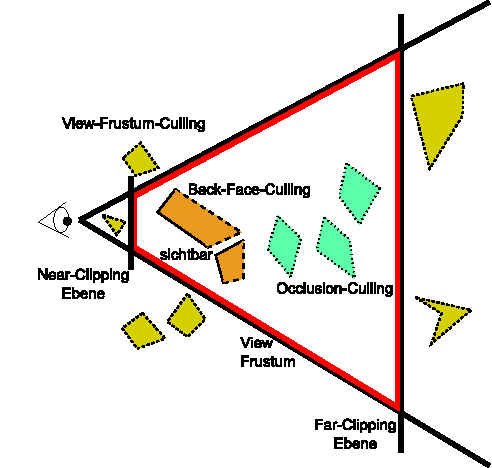
\includegraphics[scale=0.8]{images/culling.pdf}
  \caption{Verschiedene Culling-Techniken. Entfernte Geometrie ist durch gestrichelte Linien dargestellt. \textit{Quelle: nach \cite{culling}} }
  \label{fig:basics:culling}
\end{figure}
Beim Back-Face-Culling\footnote{\cite{RTR3}, Seiten 662 ff.} werden diejenigen Polygone entfernt, die vom Betrachter abgewandt sind. In Abbildung \ref{fig:basics:culling} würden bei den orangen Polygonen die vorderen Flächen gerendert, wobei die hinteren entfernt würden (gestrichelte Linien). Dabei muss jede Fläche separat auf ihre Ausrichtung überprüft werden. In dieser Arbeit wird die von OpenGL angebotene Funktion für Back-Face-Culling verwendet.\\
View-Frustum-Culling entfernt Polygongruppen, die sich außerhalb des ViewFrustums befinden. In Abbildung \ref{fig:basics:culling} wären alle gelben Flächen außerhalb des Frustums (roter Bereich) davon betroffen. Alle Objekte, die sich vollständig oder partiell im Kamerabereich befinden, müssen gerendert werden. Da die Überprüfung von mehreren Millionen Dreiecken pro Frame zeitlich zu aufwendig ist, werden in dieser Arbeit lediglich die Boundingboxen von Objektgruppen getestet. Verwendet man zusätzliche räumliche Datenstrukturen, wie Octrees (siehe \ref{sec:basics:octree}), kann das Frustum-Culling hierarchisch durchgeführt werden. Dabei wird der Baum rekursiv von der Wurzel bis zu dem Blättern durchlaufen. Liegt die Boundingbox eines Knotens vollständig im Frustum, können alle Kindknoten ohne weitere Tests ebenfalls gezeichnet werden. Liegt eine Boundingbox vollständig außerhalb des Frustums, kann der Knoten samt aller Kindknoten entfernt werden, da diese ebenfalls außerhalb des Frustums liegen. Wird eine Box jedoch von einer Grenze des Frustums geschnitten, muss zum Einen die Geometrie im Knoten gerendert und die Kindknoten weiter getestet werden. Als weitere Möglichkeit zur Optimierung kann man sich diejenigen Grenzen speichern, die eine Box schneiden. Bei folgenden Tests der Kindknoten müssen diese nur noch auf die gespeicherten Schnittflächen überprüft werden.\\
Soll vermieden werden, dass Objekte, die durch andere Polygongruppen verdeckt sind, gerendert werden, spricht man von Occlusion-Culling\footnote{\cite{RTR3}, Seiten 670 ff.}. Solche verdeckten Polygone würden in der Rendering-Pipeline transformiert, beleuchtet und anschließend gerastert, obwohl sie im fertigen Bild nicht sichtbar wären. In Abbildung \ref{fig:basics:culling} sind die grünen Objekte vollständig verdeckt. Um mehrere Objekte auf ihre Sichtbarkeit zu überprüfen, wird gegen den Tiefenbuffer (Z-Buffer) getestet. Dazu muss schon ein Teil der Szene im Tiefenbuffer gerendert sein. Dabei ist die Zeichenreihenfolge wichtig. Gerendert wird in der Regel von vorne nach hinten in Abhängigkeit vom Standpunkt des Betrachters. Wird beispielweise bei der Boeing die Außenhülle als erstes gezeichnet, kann diese als Testgrundlage im Z-Buffer verwendet werden, um die Innenräume auf Verdeckung zu überprüfen. Rendert man zuerst die Innenräume, müssen beide Teile gezeichnet werden. Die Entfernung von Objekten zur Kamera spielt ebenfalls eine Rolle. So kann eine Streichholzschachtel die Golden Gate Bridge vollständig verdecken, wenn sich der Betrachter hinreichend dicht an der Streichholzschachtel befindet. Mittlerweile lässt sich Occlusion-Culling direkt auf der Grafik-Hardware durchführen. Dazu werden Occlusion-Queries verwendet, die nach dem Test ausgeben, wie viele Pixel der Objekte sichtbar sind. Vorher können alle grafischen Effekte, wie Shader, Beleuchtung, usw. ausgeschaltet werden, um den Vorgang zu beschleunigen. Die Geschwindigkeit lässt sich noch verbessern, wenn statt der Originalgeometrie, nur Approximationen der Objekte gerendert werden. In dieser Arbeit wird Occlusion-Culling deshalb auf Boundingboxen durchgeführt. Dies kann jedoch zu falschen Testergebnissen führen. In Abbildung \ref{fig:basics:oculling} sind zwei verdeckte Objekte zu sehen. Beide befinden sich in der gleichen Boundingbox. Die Box der beiden Objekte wird beim Verdeckungstest jedoch als sichtbar markiert und sämtliche in der Box befindliche Geometrie wird gerendert. Dadurch wird zwar mehr Geometrie verschickt und gezeichnet als eigentlich sichtbar ist, was aber nicht zu Fehlern im Bild führt.
\begin{figure}
  \centering
  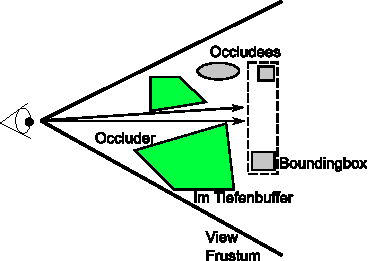
\includegraphics[scale=0.8]{images/oculling.pdf}
  \caption{Problem beim Occlusion Culling: Die Boundingbox zweier Objekte ist sichtbar, obwohl die darin enthaltenen Objekte verdeckt sind.}
  \label{fig:basics:oculling}
\end{figure}

\subsection{Datenmanagement}
\label{sec:basics:daten}
\todo[size=\small, inline]{Skizze zum $c$-Collision Protokoll? *nichtmag*}
Das $c$-Collision Protokoll wird in Kapitel \ref{chap:relwork} genauer beschrieben. In dieser Arbeit wird es verwendet, um Datenanfragen möglichst gleichmäßig im Netzwerk zu verteilen. Jedes VBO (siehe \ref{sec:basics:computergrafik}) wird zufällig und redundant im Netzwerk verteilt. Alle Anfragen von allen Renderern werden jeden Frame gesammelt. Anschließend werden diese Anfragen zu Paketen gebündelt, die ebenso viele Anfragen enthalten wie es Datenknoten im Netzwerk gibt. Das $c$-Collision Protokoll wird immer auf einem Anfragenpaket ausgeführt. Begonnen wird mit $c = 2$. Sollte in einer Runde kein weiterer Auftrag vergeben werden, obwohl noch offene Aufträge vorhanden sind, wird das $c$ erhöht. Dies wird so lange wiederholt, bis alle Aufträge aus einem Paket vergeben sind. Das $c$ wird für weitere Pakete wieder auf 2 gesetzt. Sollten innerhalb einer Paketrunde mehrere Datenknoten gleiches Anrecht auf die Bearbeitung des Auftrags haben, wird der Auftrag zufällig an einen Knoten vergeben. Dabei wird jedoch die bisherige Last an bereits vergebenen Aufträgen dieser Runde berücksichtigt. Diese Last in Form von Dreiecken wird somit als Gewichtung für das $c$-Collision Protokoll benutzt. In den Tests wurden verschiedene Seeds für die Zufallsverteilung gewählt. Innerhalb eines Tests wurde jedoch immer derselbe Seed benutzt, um das Ergebnis reproduzieren und vergleichen zu können.

Im Rahmen dieser Arbeit wurden verschiedene Typen von Rechenknoten entwickelt (siehe Kapitel \ref{chap:impl}). Die Renderknoten sind dabei für das Rendering der Kacheln zuständig. Zur Lastbalancierung der Renderknoten wurde hier eine dynamische Kachelung implementiert. Nach einer festgelegten Framezahl schicken die Renderknoten ihre gemittelten Renderzeiten für einen Frame an den Masterknoten, welcher anhand dieser dann neue Kachelgrößen vergibt. In der vorliegenden Arbeit wird ein Split-Tree verwendet, um die Kachelgrößen festzulegen. Dieser teilt, ähnlich einem KD-Tree \cite{RTR3}, den Bildschirm entlang einer Kante und die so entstandenen Kacheln ebenfalls, bis sich so viele Kacheln wie Renderer ergeben. 

\subsection{Speichermanagement}
\label{sec:basics:speicher}
Bei 3D-Szenen in Größenordnung der Boeing 777 (ca. 10 GiB) bedarf es einigen Mechanismen zur Verwaltung des Speichers. Denn obwohl in der vorliegenden Arbeit ein paralleler Out-Of-Core-Renderer entwickelt wurde, haben auch da die einzelnen Daten- und Renderknoten begrenzte Speicherressourcen. Durch die Verteilung des Render-Vorgangs auf mehrere Rechenknoten muss der Renderer nicht die gesamte Szene im Arbeitsspeicher haben. Doch auch diese Teilszenen müssen verwaltet werden. Da die Datenmengen, die jeden Frame über das Netzwerk verschickt werden, eine große Rolle bei der Rendergeschwindigkeit und der Bildkorrektheit eine große Rolle spielen, wurde in dieser Arbeit ein Caching-Mechanismus für die Renderknoten entwickelt. Dabei spielt die Cache-Verdrändung jedoch auch eine Rolle, denn der Hauptspeicher ist begrenzt. Wird ein Objekt im Verlauf des Frustum-Tests als sichtbar markiert, welches noch nicht auf dem Renderer vorhanden ist, wird es angefordert. Zwischen der Anforderung eines Objekts und dessen Eintreffen können mehrere Frames liegen. Deshalb wird beim Eintreffen eines solchen Objekts zunächst durch einen lokalen Occlusion-Test untersucht, ob das Objekt noch immer sichtbar ist. Ist es sichtbar, wird es in den Speicher der Grafikkarte gelesen (\textit{Online}), andernfalls verbleibt es lediglich im Hauptspeicher (\textit{Offline}). So ist das Objekt, sollte es in absehbarer Zeit benötigt werden, schneller verfügbar. In jedem Frame wird die gesamte Liste an verfügbaren Objekten auf Verdrängungsmöglichkeiten untersucht. Zum einen ist darauf zu achten, dass nicht zu viele Objekte im Grafik-RAM liegen, sonst wird die Simulation zu langsam. Zum Anderen sollte die gesamte Objektliste auch nicht zu lang werden, weil dies ebenfalls zulasten der Rendergeschwindigkeit geht.\\
Um dies zu regulieren, erhält jedes vorhandene Objekt einen Statuszähler. Dieser wird bei einem Statuswechsel, zum Beispiel von Offline zu Online, zurückgesetzt, andernfalls wird er in jedem Frame erhöht. Wird dabei ein gewisser Schwellwert überschritten, werden diese Objekte erneut lokal auf ihre Sichtbarkeit hin überprüft und gegebenenfalls auf Online oder Offline gesetzt. Zusätzlich erhält jedes Objekt einen Offlinezähler. Dieser wird in jedem Frame erhöht, in dem besagtes Objekt den Zustand Offline besitzt. Beim Übersteigen eines Schwellwerts wird angenommen, dass das Objekt auch in absehbarer Zeit nicht benötigt wird und das Objekt wird aus dem Cache gelöscht.
\begin{figure}
\centering
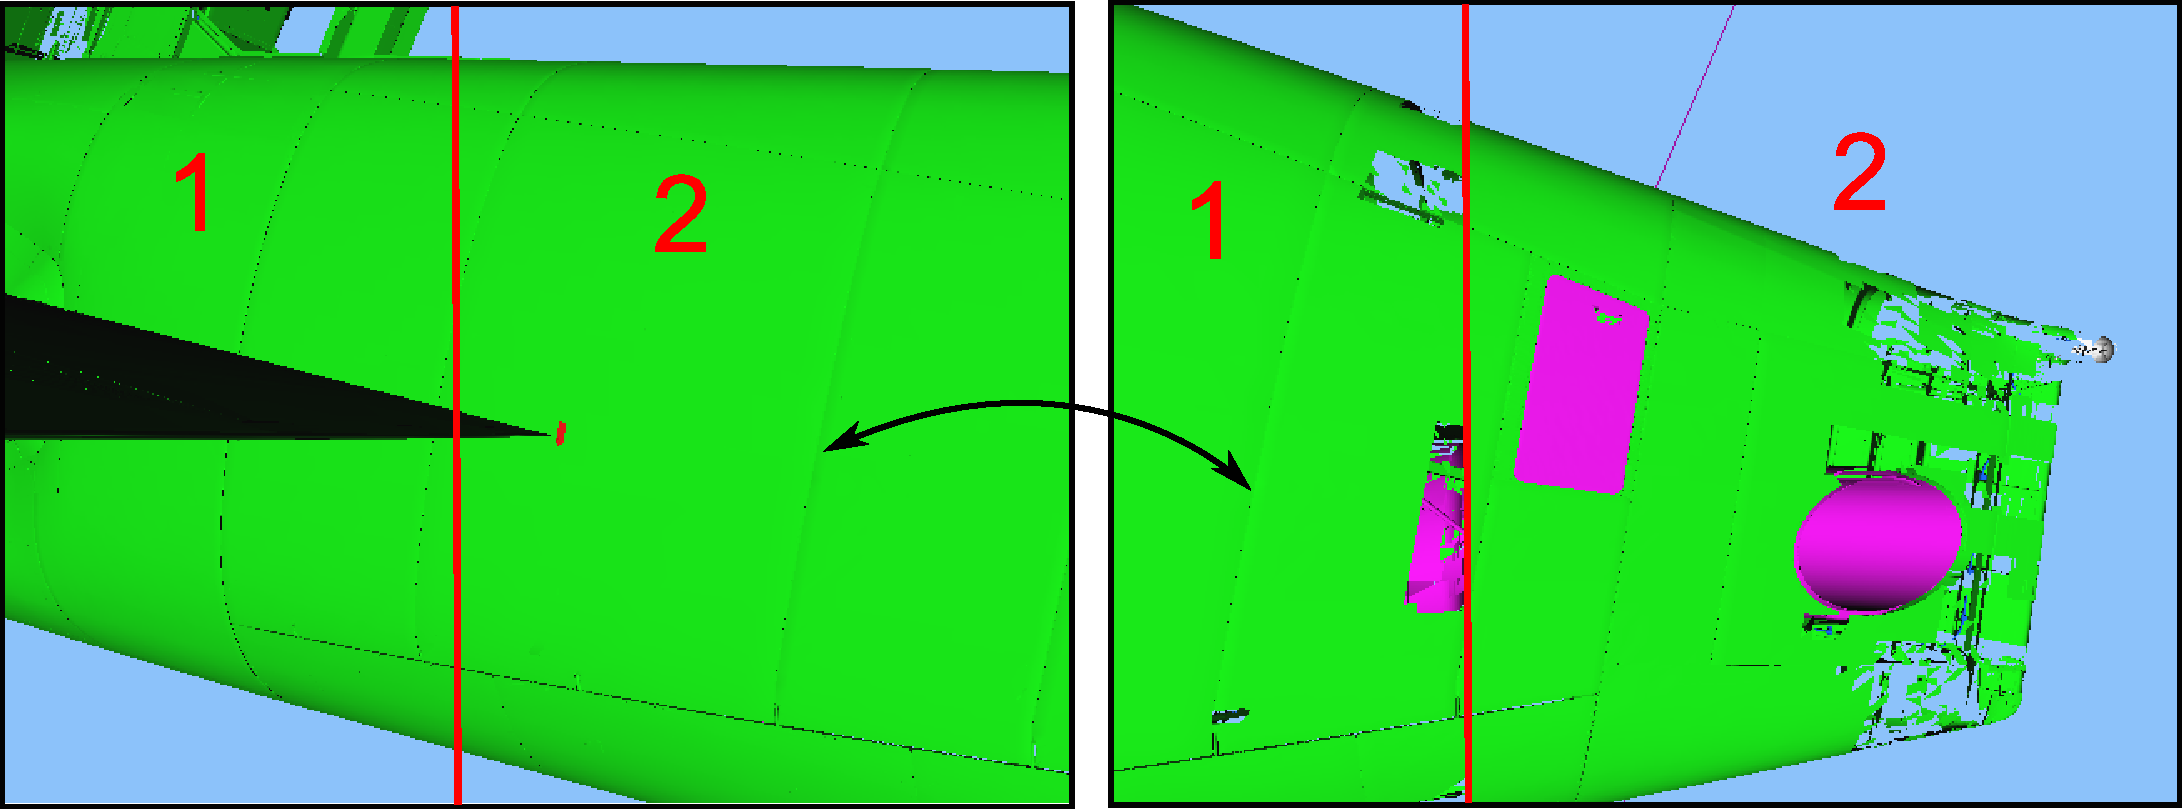
\includegraphics[scale=0.40]{images/prefetching.pdf}
\caption{\label{fig:basics:prefetching}Popping-Effekte durch schlechtes Prefetching bei einem Kameraschwenk von links nach rechts. \textit{Links: Ausgangssituation. Die Kachelrenderer 1 und 2 haben alle benötigten Daten gerendert. Rechts: Durch den Rechtsschwenk fehlen bei Renderer 1 Objekte, die zuvor Renderer 2 gerendert hat. Renderer 2 hingegen hat noch nicht alle Objekte am rechten Kachelrand geladen.}}
\end{figure}
Bei mehreren Kacheln kann ein kleiner Kameraschwenk schon dazu führen, dass Objekte, welche zuvor ausschließlich von einem Renderer dargestellt wurden, ebenfalls von einem anderen Renderer benötigt werden, oder Objekte im Randbereich angefordert werden müssen (siehe Abbildung \ref{fig:basics:prefetching}). Um diesem Effekt vorzubeugen, wird in der vorliegenden Arbeit ein Prefetching eingesetzt. Der Frustum-Test wird auf einem erweiterten Frustum durchgeführt. Jede Kachel entspricht einem Ausschnitt des vollständigen Frustums, der Test jedoch erfolgt auf einem Frustum mit einer erhöhten Brennweite und Kachelauflösung. Dadurch werden zwar Objekte an gefordert, welche außerhalb des eigentlichen Frustums liegen, aber Bildfehler beim Bewegen der Kamera können so verringert werden. Vollständig zu verhindern sind sie jedoch nicht.\\
Das ständige Reservieren und Freigeben von kleineren Speicherblöcken führt im Laufe der Zeit jedoch zu einer Fragmentierung des Hauptspeichers, weshalb in dieser Arbeit eine eigene Speicherverwaltung implementiert wurde (siehe Kapitel \ref{chap:impl}). 

\section{Approximation}
\label{sec:basics:approximation}
Approximationen in der Computergrafik haben oft zufolge, dass die Bildqualität verringert wird. Sei es, weil Objekte in Abhängigkeit zur Kameraentfernung in niedrigeren Auflösungen gerendert werden, oder dass nicht das vollständige Modell gerendert wird.
Durch das hier Frustum-Culling und Occlusion-Culling (siehe \ref{sec:basics:algos:culling}) werden Teile des Modells entfernt, welche mit einer gewissen Sicherheit nicht sichtbar sind. Da die ersten Occlusion-Tests auf den Datenknoten stattfinden, sind diese auf möglichst aktuelle Tiefenbuffer der einzelnen Renderer angewiesen. Da das Auslesen und Schreiben von Tiefeninformationen jedoch Zeit in Anspruch nimmt, wird dieses Update nur nach einer gewissen Frame-Anzahl vorgenommen und das nur, wenn die Kamera bewegt wurde. Dadurch kommt es zu Ungenauigkeiten bei den Verdeckungstests, es wird aber angenommen, dass diese immer noch hinreichend genau sind. \\
Die Traversierung des Sampletrees wird abgebrochen, unter der Annahme, dass die Geometrie in den Kindknoten nicht mehr als ein Pixel im fertigen Bild beträgt. Dadurch werden sichtbare Teile des Modells nicht gerendert. Der Sampletree nähert diese Teile an, indem dort Dreiecke in höhere Hierarchiebenen verschoben wurden (siehe \ref{sec:basics:sampletree}).

Außerdem wird eine möglichst hohe Bildrate gegenüber einem fehlerfreien Bild bevorzugt. Es gibt Situationen in denen die Bewegung der Kamera zwar unmittelbar ausgeführt wird, die benötigten geometrischen Objekte aber erst nach und nach bei den Renderern eintreffen (Popping-Artefakte). Eine weitere Approximation stellt die Beschränkung der Cachegröße und die Verdrängung von Objekten aus dem Cache dar. Werden Objekte aus dem Cache verdrängt, die unmittelbar danach wieder angefordert werden, kann es durch die Latenz im Netzwerk zwischen Anfragen und deren Antworten zu Popping-Effekten kommen. (siehe auch \ref{sec:basics:speicher}). 
